\documentclass[11pt]{article}%

\usepackage{styles/style}

\begin{document}
\section{Contraction Ratio with Uncertainty in Regular Polygons}

\begin{figure}[!h]
  \centering
  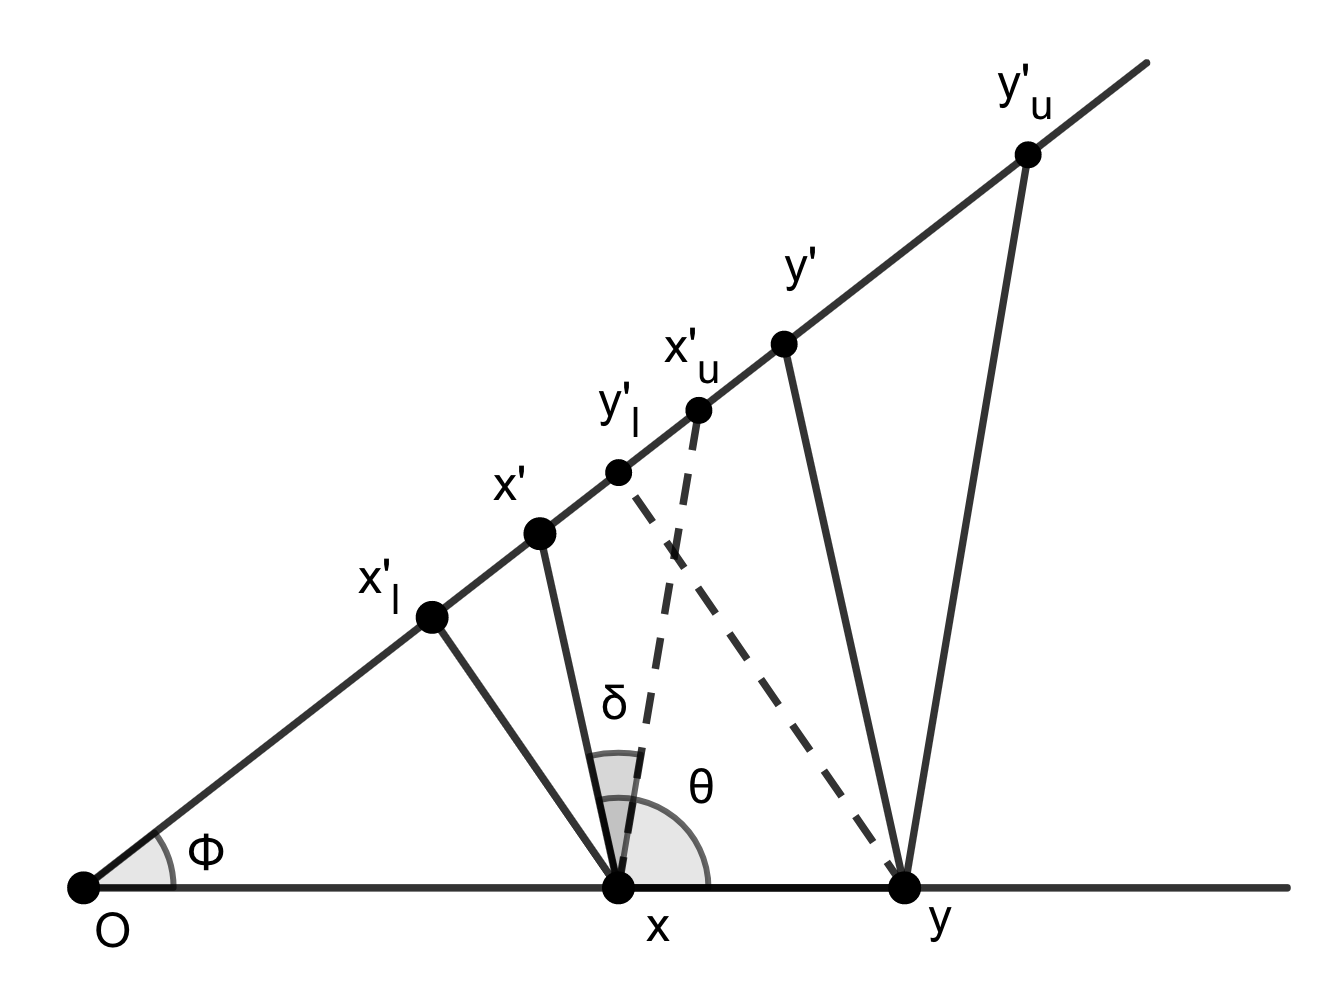
\includegraphics[width=0.5\linewidth]{uncertainty_bounce.png}
  \caption{Bounce with uncertainty}
  \label{fig:uncertain_bounce}
\end{figure}
Suppose our environment is a regular polygon with edge length $1$. To compute fix angle bouncing for an interval on the boundary, we can consider the individual bounce of the end points of the interval and the length of the range at each bounce will be the difference between the end points positions. When we add a fix $\delta$ uncertainty to such bounce, i.e., instead of bouncing at $\theta$, the robot chooses an arbitrary angle in $[\theta - \delta, \theta + \delta]$, the worse case results is when the end point on the right bounces at $\theta - \delta$ and the end point on the left bounces at $\theta + \delta$, as shown by $y'_u$ and $x'_l$ in figure~\ref{fig:uncertainty_bounce}. 
\begin{figure}[!h]
  \centering
  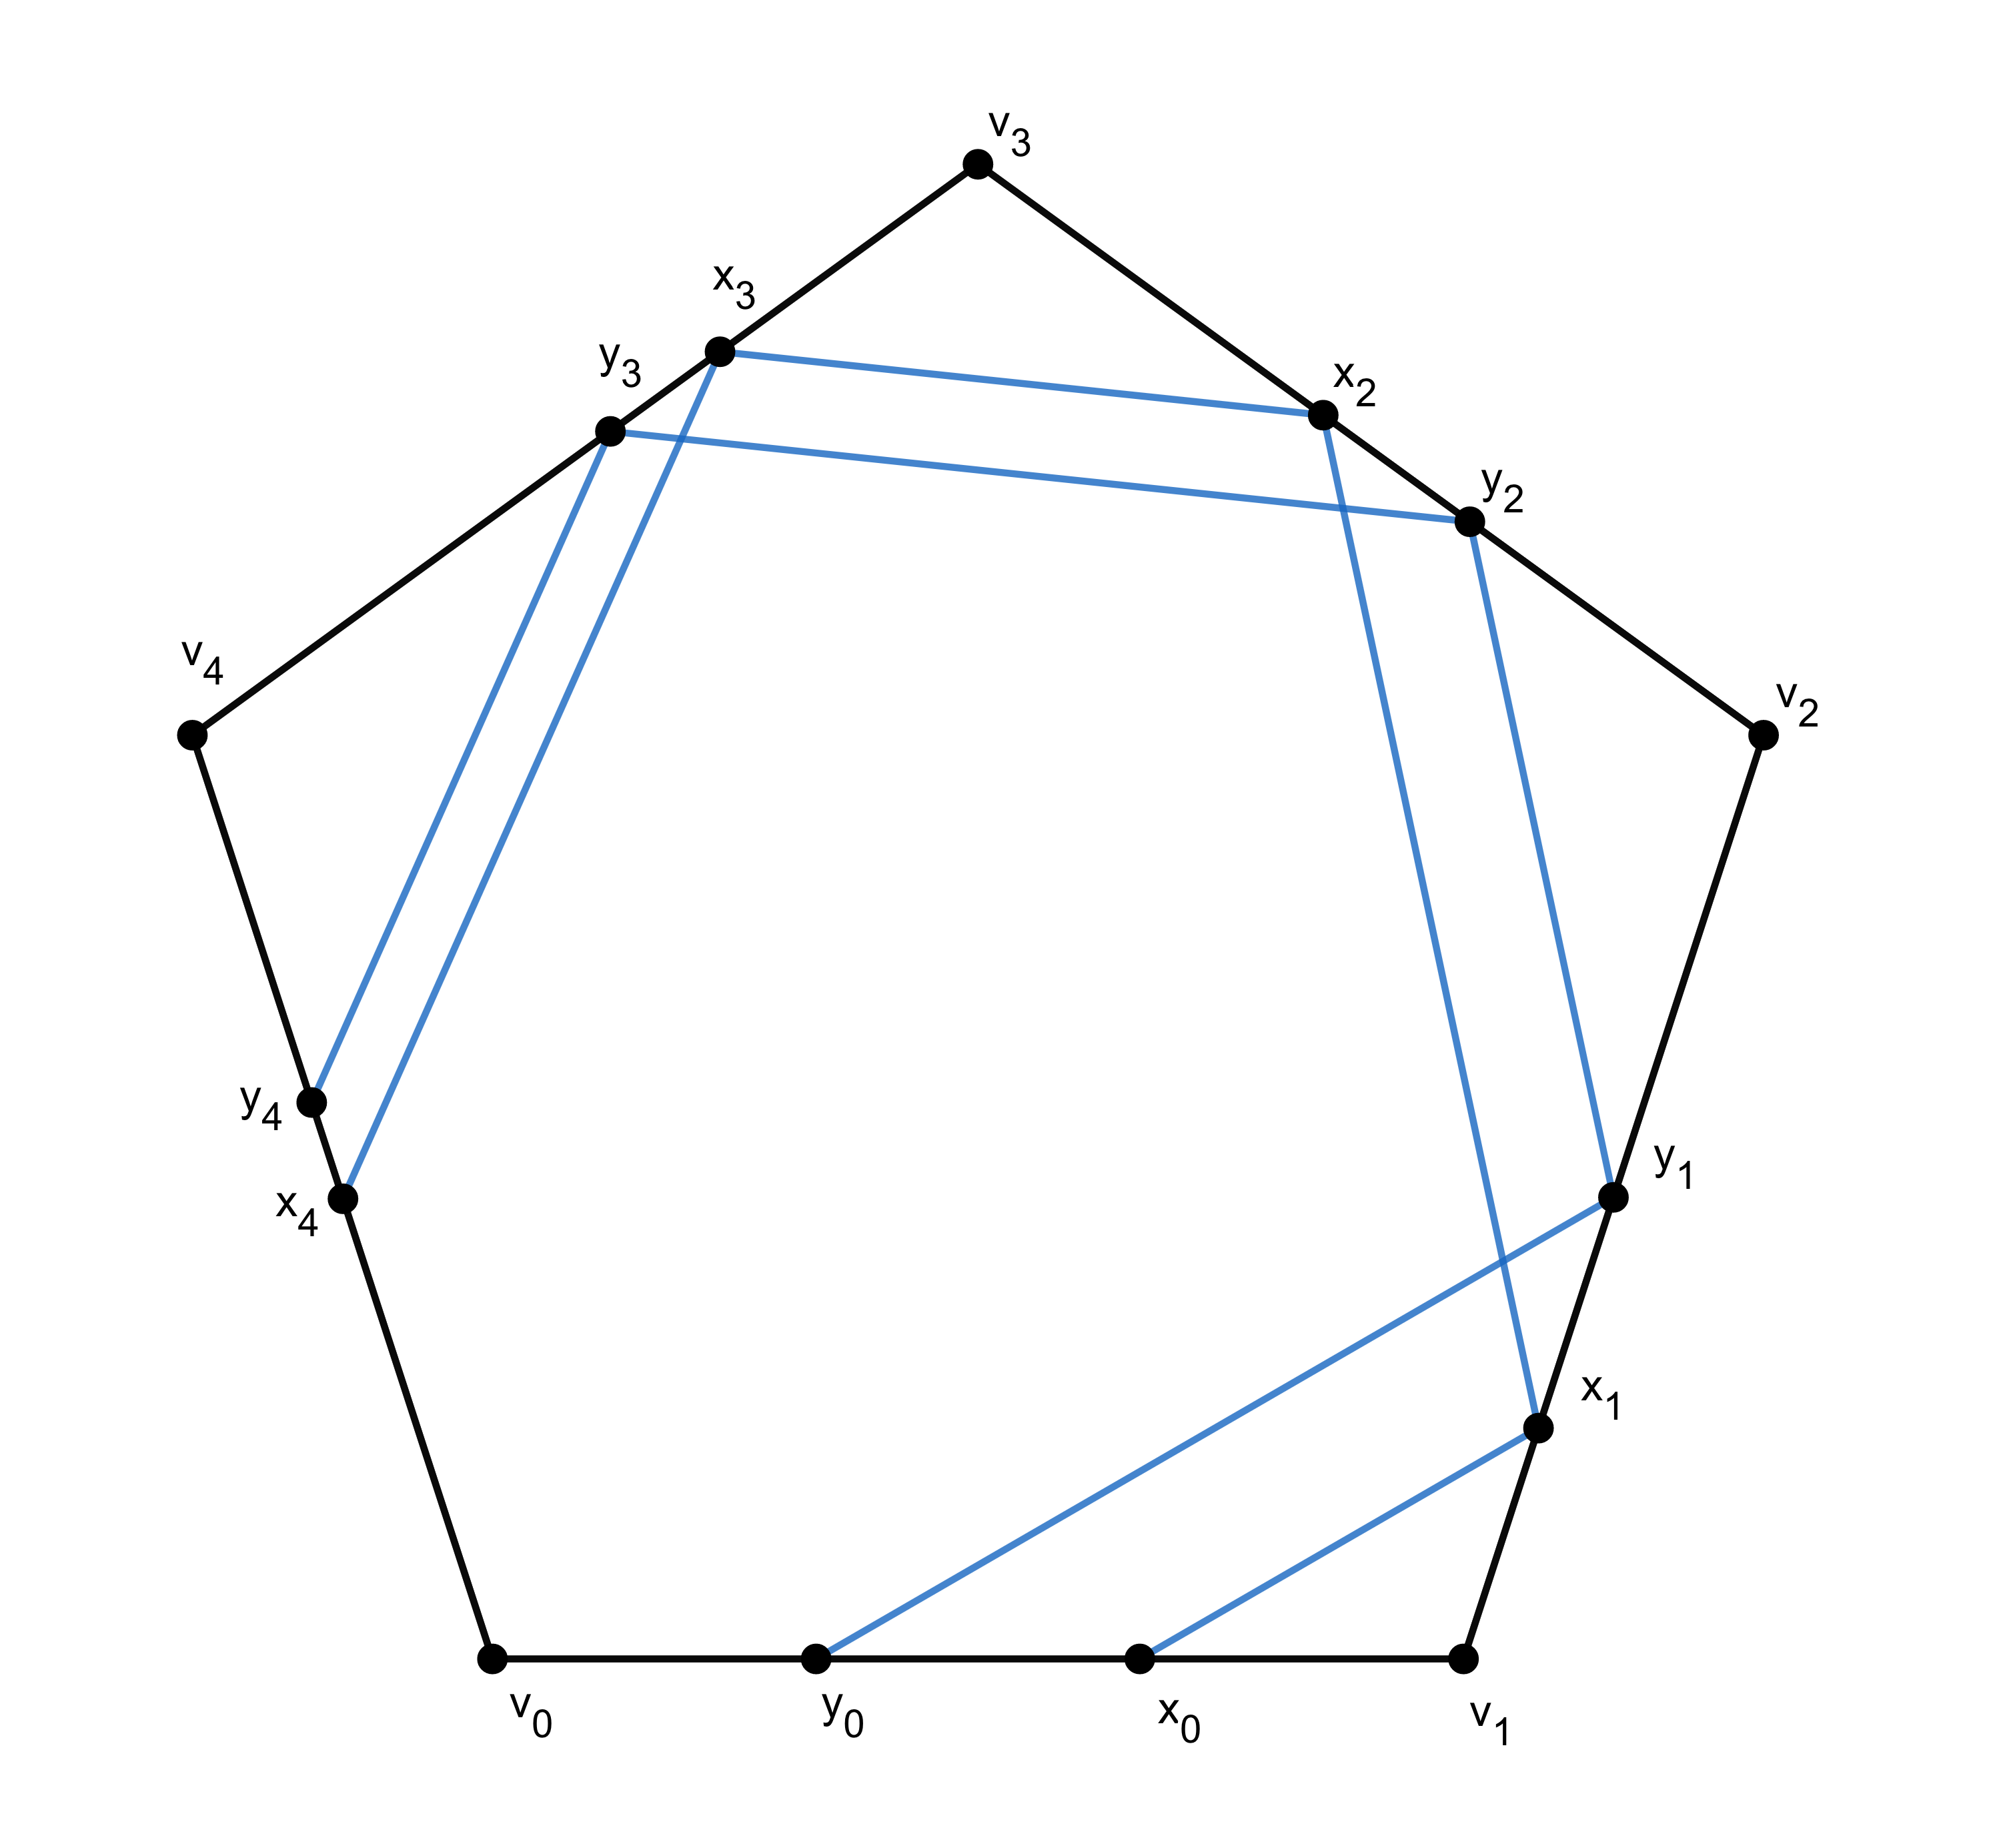
\includegraphics[width=0.5\linewidth]{alternate_side.png}
  \caption{The end points of an interval alternate between being the right end point and the left end point.}
  \label{fig:alternate_side}
\end{figure}
In a sequence of bounce for a fix interval, the end points of the interval alternates between being the right end point and the left end point, as shown by the sequence of $x_i$ and $y_i$ in figure~\ref{alternate_side}.

When the bounce angle is $\theta + \delta$, we have $x_{t} / (1-x_{t-1}) = \frac{\sin(\theta + \delta)}{\sin(\phi - \theta - \delta)} \eqqcolon r_{1}$; similarly, when the bounce angle is $\theta - \delta$, we have $x_{t} / (1-x_{t-1}) = \frac{\sin(\theta - \delta)}{\sin(\phi - \theta + \delta)} \eqqcolon r_{2}$. So $x_{t} = r_{1}(1-x_{t-1})$ or $r_{2}(1-x_{t-1})$ depending on whether $x_{t-1}$ is a left end point or right end point. 
\begin{figure}[!h]
  \centering
  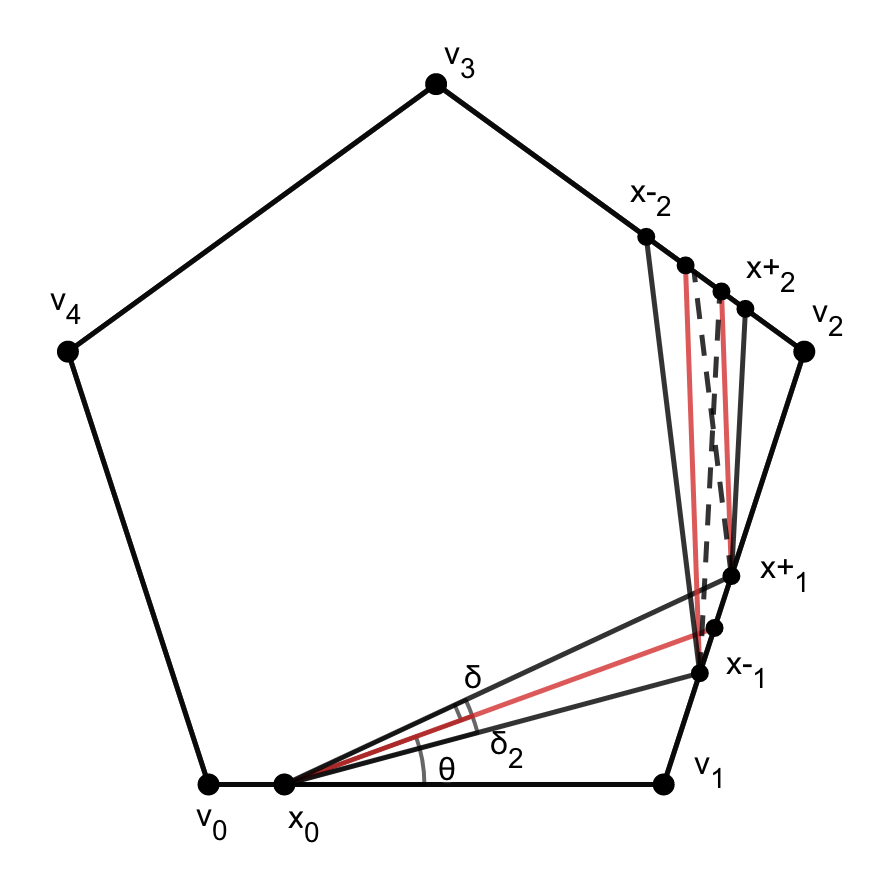
\includegraphics[width=0.5\linewidth]{plus_minus_bounce.png}
  \caption{The $x^{+}$ sequence starts with $\theta+\delta$ bounce and the $x^{-}$ sequence starts with $\theta-\delta$ bounce.}
  \label{fig:plus_minus_bounce}
\end{figure}
Let $x^{+}$ denotes the sequence of positions that started from $x_{0}$ with a $\theta+\delta$ bounce, and $x^{-}$ denotes the sequence of positions that started from $x_{0}$ with a $\theta-\delta$ bounce, as shown in figure~\ref{fig:plus_minus_bounce}. 

We can show by induction (or unrolling) that 
\[x^{+}_{t} = \frac{r_{1}(1-r_{2})(1-(r_{1}r_{2})^{n})}{1-r_{1}r_{2}} + (-1)^{t}r_{1}^{\floor{t/2}}r_{2}^{\ceil{t/2}}x_0\]
\[x^{-}_{t} = \frac{r_{2}(1-r_{1})(1-(r_{1}r_{2})^{n})}{1-r_{1}r_{2}} + (-1)^{t}r_{1}^{\ceil{t/2}}r_{2}^{\floor{t/2}}x_0\]


If $r_{1}r_{2}<1$, then $x^{+}_{\infty} = \frac{r_{1}(1-r_{2})}{1-r_{1}r_{2}}, x^{-}_{\infty} = \frac{r_{2}(1-r_{1})}{1-r_{1}r_{2}}, |x^{+}_{\infty} - x^{-}_{\infty}| = |\frac{r_{1}-r_{2}}{1-r_{1}r_{2}}|$. 

Remark: since the term containing the start position $x_{0}$ vanishes, the results for $t = \infty$ does not depends on the initial condition. Even if the start position for the $x^{+}, x^{-}$ sequence are different, we will still have the same convergence. 
\end{document}